\begin{figure}
  \centering
    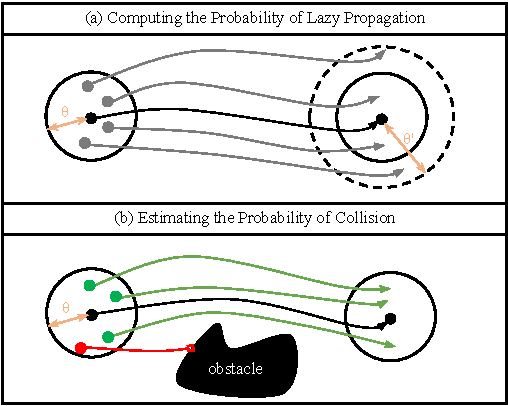
\includegraphics[width=\columnwidth,height=0.8\columnwidth]{assets/pert_mod.pdf}
  \caption{Perturbing the start state of an edge $e_i \in \mathcal{E}$ (black arrow) by a maximum of $\theta$ and applying $e_i.u$ for duration $e_i.\Delta t$ results in a perturbed end state ($\hat{q}_f$). Applying multiple random perturbations for $e_i$ (grey arrows in (a), green and red arrows in (b)) allows us to estimate $e_i.P_{\text{lazy\_prop}} = Pr(\|\hat{q}_f - e_i.q_f\|_2 < \theta) = 2/4$ and $e_i.P_{\text{collision}} = 1/4$ for the provided example. We repeat this process for all edges in $\mathcal{E}$ to integrate lazy approaches to simulation and collision checking in \textsl{LazyBoE}.}\label{fig:pert_analysis}
\end{figure}

\section{Methods}\label{sec:methods}

In this section, we present \textsl{LazyBoE}, our multi-query kinodynamic motion planner. The planner relies on two key contributions: 1) a method for generating a bundle of edges in order to provide a discrete approximation to the robot's state and control spaces (\cref{sec:methods-eb_construction}), and 2) a quantification of lazy propagation and collision probabilities to reduce planning time (\cref{sec:methods-perturbation}). These pieces enable us to design and implement a planner that defers computation in the form of simulation and collision-checking until there is a viable path that minimizes a heuristic value (\cref{sec:methods-planner}).

\subsection{Problem Setup}

We formalize the problem of kinodynamic motion planning using edge bundles similarly to \cite{shome2021asymptotically}.
The robot state space $\mathcal{Q} \subset \mathbb{R}^m$ is defined where $q \in \mathcal{Q}$ represents the joint angles of an $m$-dimensional robot. The control space $\mathcal{U} \subset \mathbb{R}^m$ contains elements $\dot{q} \in \mathcal{U}$ that represent joint velocities.
An \textsl{edge bundle} is a set of disconnected edges generated by applying randomly sampled control parameters to random robot states for random time durations, thereby connecting random start states to resultant end states:
\begin{center}
$\mathcal{E} = \{(q_0, \boldsymbol{\dot{q}}, \Delta t, q_f) \mid q_0, q_f \in \mathcal{Q}, \hspace{3pt} \boldsymbol{\dot{q}} \in \mathcal{U}\}$
\end{center}
such that $f(q_0, \boldsymbol{\dot{q}}) = q_f$, where $f(\cdot)$ defines the forward dynamics model of the robot and $\boldsymbol{\dot{q}} = (\dot{q}_0, \cdots, \dot{q}_{f-1})$ represents a sequence of joint velocities. The $i$-th edge is denoted as $e_i$ and defined as the tuple $(q_0^i, \boldsymbol{\dot{q}^i}, \Delta t^i, q_f^i)$.
The objective of \textsl{LazyBoE} is to find a continuous, collision-free trajectory
$$\pi(t) : [0,1] \rightarrow \mathcal{Q}_{\text{free}} \subseteq \mathcal{Q}, \quad \pi(0) = q_0, \quad \pi(1) = q_f$$
through the state and control space discretization enabled by $\mathcal{E}$, while respecting the dynamics constraints $\mathcal{D}$ of the robot.

\subsection{Edge Bundle Construction with the Robot Dynamics Model}\label{sec:methods-eb_construction}

The backbone of our planner lies in constructing a discrete approximation of the robot's state and control spaces, as a result capturing the nuances of real-world dynamics including nonlinearities like joint friction. Defined as a bundle of edges $\mathcal{E}$, this approximation is a collection of valid, disconnected, and randomly generated forward rollouts of the robot dynamics model over a variable duration $\Delta t$. This method of edge generation with a sampled duration is known as Monte Carlo propagation and ensures the preservation of asymptotic optimality in kinodynamic planning algorithms \cite{kunz2015kinodynamic}.
In order to enable uniform and rapid exploration of the control space, we propagate a sequence of randomly-sampled joint velocity actions, $\boldsymbol{\dot{q}} = (\dot{q}_0, \cdots, \dot{q}_f) \in \mathcal{U}$, from a randomly sampled state, $q \in \mathcal{Q}$. In addition to providing a broader local reachability range (and as a result expanding the explored volume in the state space) from a given state, varying joint velocities over a single propagation leads to longer-duration edges as it prevents the robot from becoming locally ``locked'' along fixed controls.
Moreover, it is necessary that these Monte Carlo propagations are collision-free and obey the Euler-Lagrange robot dynamics model $\mathcal{D}$ to ensure validity in real-world execution. Our approach to bundle generation can be extended to other robot embodiments as long as a valid dynamics model is provided.

As an example, we focus on one particular embodiment and use an analytically-derived and empirically-tuned dynamics model for the 7 degrees-of-freedom (DoF) Franka Emika Panda arm \cite{Gaz2019}. This analytical model is defined as
$\tau(q, \dot{q}, \ddot{q}) = M(q)\ddot{q} + C(q, \dot{q})\dot{q} + g(q) + f(\dot{q})$,
where $q$, $\dot{q}$, $\ddot{q}$, and $\tau$ are $7\times1$ vectors representing the robot's joint angles, velocities, accelerations, and torques, respectively. $M$ is a symmetric, positive-definite $7\times7$ joint inertia matrix, $C$ is a $7\times1$ matrix that captures the Coriolis and centrifugal effects caused by robot motion, $g$ is a $7\times1$ vector encapsulating the torque required by each motor to counteract gravitational forces, and $f$ is a $7\times1$ vector that quantifies the torques necessary to counteract friction at the joints. The model is used to verify whether the propagated joint velocity sequence $\boldsymbol{\dot{q}}$ obeys the robot torque limits.

Furthermore, validating an edge involves three classes of checks: collision checks, robot state limit checks, and continuity checks (\cref{algo:lazyboe}, Lines 20-22).
Acceptable ranges for the state and control variables and additionally, dynamics quantities are defined as $q_{min} < q < q_{max}$, $\dot{q}_{min} < \dot{q} < \dot{q}_{max}$, $\ddot{q}_{min} < \ddot{q} < \ddot{q}_{max}$, and $\tau_{min} < \tau < \tau_{max}$.
In addition, the dynamics simulations must obey continuity constraints due to the stringent control requirements of this robot.
For a given static environment, edges are validated to be free of self-collision and environmental collisions via geometric collision-checking algorithms. This incurs a one-time cost since the edges can be used lazily for a significant portion of our motion planning process.
We next explain how we can compute useful quantities from this generated edge bundle to enable lazy kinodynamic planning.

\begin{algorithm}\footnotesize
\caption{LazyBoE}\label{algo:lazyboe}
  \KwIn{Start State $q_0$, Goal Region $\mathcal{Q}_{goal}$, Edge Bundle $\mathcal{E}$, Neighborhood Radius $\theta$}
  \KwOut{Path $\pi$}
  $\pi \leftarrow \emptyset$\\
  $\mathcal{V} \leftarrow \{q_0\}$\\
  \While{$\mathcal{V} \neq \emptyset$} {
    \tcp{equivalent to SELECT(.) in \cite{shome2021asymptotically}}
    $v \leftarrow \text{PICK\_NODE}(\mathcal{V})$\\
    \tcp{update $\pi$ to lower cost path}
    \If{$v \in \mathcal{Q}_{goal}$ \textbf{and} $!\text{IS\_LAZY}(\text{EDGE\_TO}(v))$} {
        \If{cost$(\pi) > $ cost$(\text{PATH\_TO}(v))$} {
            $\pi \leftarrow \text{PATH\_TO}(v)$
        }
    }
    \If{IS\_LAZY(EDGE\_TO(v))} {
        $\mathcal{E}_{\text{neighbor}} \leftarrow \text{RADIAL\_NN}(v, \theta / 2, \mathcal{E})$
    }
    \Else {
        $\mathcal{E}_{\text{neighbor}} \leftarrow \text{RADIAL\_NN}(v, \theta, \mathcal{E})$
    }
    %\\
    $\mathcal{V}_{\text{next}} \leftarrow \emptyset$\\
    \ForEach{$e \in \mathcal{E}_{\text{neighbor}}$} {
        $P_{\text{select}} \leftarrow (1 - e.P_{\text{collision}}) * e.P_{\text{lazy\_prop}}$\\
        $\text{apply\_lazy\_prop} \leftarrow rand() < P_{\text{select}}$\\
        \If{apply\_lazy\_prop} {
            $\mathcal{V}_{\text{next}} \leftarrow \mathcal{V}_{\text{next}} \cup e.q_f$\\
        }
        \ElseIf{!apply\_lazy\_prop \textbf{or} $\text{!IS\_LAZY(EDGE\_TO(v))}$ \textbf{or} (IS\_LAZY(EDGE\_TO(v)) \textbf{and} SHOULD\_TERMINATE\_LAZY())} {
            \tcp{simulate}
            $e_{new} \leftarrow f(v, e.u, e.\Delta t)$\\
            \If{$\text{COLLISION\_FREE}(e_{new})$ \\
   \textbf{and} $\text{WITHIN\_LIMITS}(e_{new})$ \\
   \textbf{and} $\text{IS\_CONTINUOUS}(e_{new})$} {
                $\mathcal{V}_{\text{next}} \leftarrow \mathcal{V}_{\text{next}} \cup e_{new}.q_f$
            }
        }
    }
    $\mathcal{V} \leftarrow \mathcal{V} \cup \mathcal{V}_{\text{next}}$

  }
  \textbf{return} $\pi$ 
\end{algorithm}


\subsection{Edge Perturbation for Lazy Propagation and Collision-Checking}\label{sec:methods-perturbation}

The task of generating an edge bundle that uniformly samples the state and control spaces of a robot is a computationally intensive process, particularly in the case of a high-DoF robot and increased environment complexity.
A substantial part of this computational workload is incurred again during the planning stage, where edges emerging from $\theta$-regions around planning tree nodes undergo simulation and collision checks \cite{shome2021asymptotically}. This $\theta$ is dependent on state-space dimensions and denotes the maximum level of similarity in the state space, thereby bounding the set of valid controls.
Additionally, the greedy, heuristic-biased search strategy used by the BoE planner has the potential to get stuck in local minima, thereby necessitating a method for quickly evaluating these greedy paths without simulating them entirely. This motivates the need for lazy approaches to simulation and collision-checking in the kinodynamic setting.
More specifically, we need to address the following two questions for each edge $e_i \in \mathcal{E}$:
\begin{enumerate}
    \item Can $e_i$ be lazily propagated instead of undergoing a full simulation?
    \item What is the probability that a lazily propagated edge will result in a collision?
\end{enumerate}

We approach the answers to these questions empirically by conducting a perturbation analysis on each edge in the bundle. A disturbance $\Delta q$ in the range $(0, \theta]$ is added to the start state for each edge. The resultant end state for an $e_i$ is computed as $\hat{q}_f^i = f(q_0^i + \Delta q, \boldsymbol{\dot{q}}^i)$. In the limit that the number of perturbations for each edge ($p$) approaches infinity, we are able to accurately estimate both the maximum error in the end state, $\Delta q_f^i = \text{max}(\|e.\boldsymbol{q}_f - \hat{\boldsymbol{q}}_f)\|_2$), and the potential collision likelihood.
To address the first question, an edge viable for lazy propagation is characterized as one that confines the end-state error within the region radius $\theta$, so that viable edges for the next level of propagations can be picked from this fixed $\theta$-neighborhood.
However, this criterion is subjected to a more stringent requirement, as depicted in \cref{fig:theta_over_2}, i.e., the end-state error for $e_i$ must be confined to $\theta / 2$ if $e_i$ undergoes lazy propagation to ensure the worst-case error between its real simulation and the following connection to the lazy edge is $\theta$.
Put differently, the probability that an edge can be lazily propagated $P_{\text{lazy\_prop}}^i = Pr(\Delta q_f^i < \theta / 2)$ is the ratio of the number of valid (collision-free and dynamically-feasible) perturbations for which the maximum end state error is $\theta / 2$ to the total number of valid perturbations, $p_{valid}$ (\cref{fig:pert_analysis}a).
Similarly, in response to the second question, we can quantify the probability that an edge will collide when lazily propagated, i.e., $P_{\text{collision}}^i = Pr(e_i \text{ collides})$, as the ratio of the number of edges that collide to the total number of perturbations $p$ (\cref{fig:pert_analysis}b). This is in contrast to prior work which only considers lazy collision checking in the geometric planning domain and takes a deterministic approach, iteratively discarding edges that are not collision-free \cite{kavraki2000path,hauser2015lazy}. The neighborhood-based control propagation in our work allows for a more nuanced and stochastic approach to lazy collision checking by allowing edges to be re-explored, potentially uncovering paths that would be prematurely eliminated by deterministic methods. In this work, we primarily deal with self-collisions and environmental collisions between the robot and its surrounding environment.
These two probability values for each edge extend the definition of an edge bundle $\mathcal{E}$ to the following:
\begin{center}
$\mathcal{E} = \{(q_0, \boldsymbol{\dot{q}}, \Delta t, q_f, P_{\text{lazy\_prop}}, P_{\text{collision}}) \mid q_0, q_f \in \mathcal{Q}, \hspace{3pt} \boldsymbol{\dot{q}} \in \mathcal{U}\}$
\end{center}

These two metrics, associated with each edge, are used to guide the planner by deciding when to apply lazy methods for faster planning times.

\begin{figure}
  \centering
    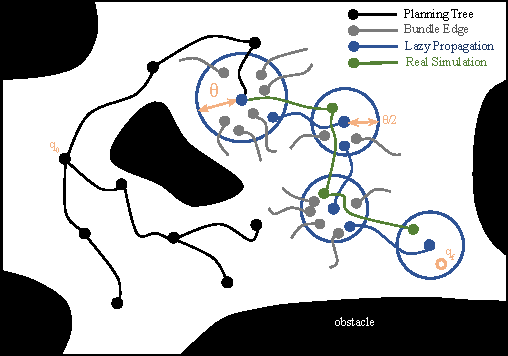
\includegraphics[width=\columnwidth,height=0.7\columnwidth]{assets/theta_over_2.pdf}
  \caption{\textsl{LazyBoE} can lazily propagate a series of edges from $\mathcal{E}$ (shown in \textsl{grey}) in a way that minimizes heuristic cost. After a lazy candidate path is found (\textsl{blue}), a full simulation and collision check is performed along this path (\textsl{green}) to extend the planning tree (\textsl{black}). To ensure the highest rate of success when performing simulation on lazy paths, neighborhood lookup is restricted to $\theta / 2$ for lazy search to allow, in the worst case, the maximum error between the end of a simulated edge and the start of the next lazy edge to be $\theta$.}\label{fig:theta_over_2}
\end{figure}

\subsection{Kinodynamic Motion Planner}\label{sec:methods-planner}
In order to reduce the computational costs associated with dynamics simulation and collision checking, we present a lazy approach for exploring the space of edge bundles $\mathcal{E}$, deferring computation until a viable, low cost approximation to a true candidate path has been found.
Our method, termed \textsl{LazyBoE}, builds upon the design decisions laid out in the BoE planner \cite{shome2021asymptotically}. In addition, it leverages the computed probabilities $P_{\text{lazy\_prop}}$ and $P_{\text{collision}}$ and combines them into the probability of selecting an edge for lazy propagation as $P_{\text{select}} = (1 - P_{\text{collision}}) * P_{\text{lazy\_prop}}$ (\cref{algo:lazyboe}, Line 14). This encourages edges with a lower collision probability to be propagated first, while also promoting lazy propagation. Since the edges are evaluated probabilistically, they can be used more than once, adding diversity and breadth to exploration, countering the downsides of the greedy approach as taken by the BoE planner. Stochasticity thereby avoids local minima and oscillation issues in greedy search.

In the ideal case scenario, all edges can be lazily propagated, enabling us to search through the edge bundle until the goal is reached and doing a real propagation on the shortest path from start to goal. However, this does not hold due to real simulations that may lead to end states beyond the neighborhood radius $\theta < \theta'$ (\cref{fig:pert_analysis}a), thereby resulting in $P_{\text{lazy\_prop}} < 1$ for many edges. Therefore, it becomes important to identify the termination conditions for defining when to stop lazy propagation. These termination conditions (as defined by SHOULD\_TERMINATE\_LAZY() in \cref{algo:lazyboe}, Line 18) are two-fold: i) heuristic value, in our case, the distance to goal state, starts increasing, or; ii) lazy propagation path reaches the goal region $\mathcal{Q}_{goal}$.
As a result, simulation along the lazy path is triggered when these conditions hold, if the preceding edge is not a lazy one, or with probability $1 - P_{\text{select}}$ (\cref{algo:lazyboe}, Line 18).
Next, we demonstrate how these lazy approaches lead to lower planning times and higher success rates in comparison to baseline kinodynamic motion planning algorithms.

